\documentclass{article}
\linespread{1.3}
\usepackage[margin=50pt]{geometry}
\usepackage{amsmath, amsthm, amssymb, amsthm, tikz, fancyhdr}
\pagestyle{fancy}
\renewcommand{\headrulewidth}{0pt}
\newcommand{\changefont}{\fontsize{15}{15}\selectfont}

\newcommand{\field}[1]{\mathbb{#1}}
\newcommand{\1}{\mathbf{1}}
\newcommand{\E}{\mathbb{E}} 
\renewcommand{\P}{\mathbb{P}}
\newcommand{\R}{\field{R}} % real domain
% \newcommand{\C}{\field{C}} % complex domain
\newcommand{\F}{\field{F}} % functional domain

\newcommand{\T}{^{\textrm T}} % transpose

\def\diag{\text{diag}}

%% operator in linear algebra, functional analysis
\newcommand{\inner}[2]{#1\cdot #2}
\newcommand{\norm}[1]{\left\|#1\right\|}
\newcommand{\twonorm}[1]{\|#1\|_2^2}
% operator in functios, maps such as M: domain1 --> domain 2
\newcommand{\Map}[1]{\mathcal{#1}}
\renewcommand{\theenumi}{\alph{enumi}} 

\newcommand{\Perp}{\perp \! \! \! \perp}

\newcommand\independent{\protect\mathpalette{\protect\independenT}{\perp}}
\def\independenT#1#2{\mathrel{\rlap{$#1#2$}\mkern2mu{#1#2}}}
\newcommand{\vct}[1]{\boldsymbol{#1}} % vector
\newcommand{\mat}[1]{\boldsymbol{#1}} % matrix
\newcommand{\cst}[1]{\mathsf{#1}} % constant
\newcommand{\ProbOpr}[1]{\mathbb{#1}}
\newcommand{\points}[1]{\small\textcolor{magenta}{\emph{[#1 points]}} \normalsize}
\date{{}}

\fancypagestyle{firstpageheader}
{
  \fancyhead[R]{\changefont Michael Huang \\ CSE 446 \\ Homework 1}
}

\begin{document}

\thispagestyle{firstpageheader}

\section*{A.0}
{\Large 

\subsection*{a.}

Bias describes how well a model matches its original training set, while Variance describes how much a model will change when we select different data to train on. \\ \\
The bias-variance tradeoff describes how there is an inverse relationship between bias and variance for a model; that is, we have lower model variance, bias tends to increase, but when we decrease bias, we tend to have higher variance. 

\subsection*{b.}

Typically, with greater model complexity, we have a greater range of data which means we have greater variance, but also lower bias as we typically are fitting on less of the training set. \\
In the same way, with lower model complexity, we have less key data which means there will be a lower variance with fewer options for training data sets, but greater bias as well.

\subsection*{c.}

False. The bias of a model is defined on a single selection of training data, so this doesn't change with more data.

\subsection*{d.}

False. Typically, adding more training data should increase the variance of a model with more options of data to train on.

\subsection*{e.}

False. With less features used to represent the data, this means that we essentially have fewer parameters, which means that we will have more issues generalizing since it is more difficult to tell the trends in the data.

\subsection*{f.}

We should only use the train set to tune hyperparameters. We should only use the test set to test our model, and using it to tune hyperparameters runs a higher risk of overfitting.

\subsection*{g.}

False. The training error is evaluated on the data it trained on itself, while the true error evaluates on all the data in the dataset, so the training error will not be an accurate overestimate.
% The training error of a function on the training set usually is too optimistic when it comes to estimating the true error.
% The training error of a function provides an overestimate of the true error?
% Usually, hard to tell whether is over/under right?

}

\section*{A.1}
{\Large

\subsection*{a.}

We aim to derive an expression for the maximum likelihood estimate of $\lambda$ in the context of the Poisson distribution in terms of $x_1, \dots, x_5$. We know that $\text{Poi}(x|\lambda) = e^{-\lambda}\frac{\lambda ^x}{x!}$, by definition. Since these observations are iid, to find the likelihood function, we simply multiply: \\ \\
$L(\lambda; x_1, \dots, x_5) = \prod_{i=1}^{5} f(x_i;\lambda) = \prod_{i=1}^{5} e^{-\lambda} \frac{\lambda^{x_i}}{x_i!} $ \\ \\
We can make things easier by taking the log-likelihood function, since the maximizer is the same for both the likelihood and log-likelihood function: \\ \\
$\text{ln } L_n(\theta) = \text{ln} (\prod_{i=1}^{5} e^{-\lambda} \frac{\lambda^{x_i}}{x_i!}) $ \\
$= \prod_{i=1}^{5} \text{ ln}(e^{-\lambda} \frac{\lambda^{x_i}}{x_i!}) $ \\
$= \sum_{i=1}^{5} \text{ ln}(e^{-\lambda} \cdot \lambda^{x_i} \cdot \frac{1}{x_i!}) $ \\
$= \sum_{i=1}^{5} \text{ ln}(e^{-\lambda}) + \text{ln}(\lambda^{x_i}) - \text{ln}(x_i!) $ \\
$= \sum_{i=1}^{5} -\lambda + x_i\text{ln}(\lambda) - \text{ln}(x_i!) $ \\
$= -5\lambda + \sum_{i=1}^{5} x_i\text{ln}(\lambda) - \text{ln}(x_i!) $ \\ \\
By definition, we aim to find $\widehat{\lambda}_{MLE} = \text{arg max}_{\lambda}L_n(\lambda) = \text{arg max}_{\lambda} \text{ ln }L_n(\lambda)$. We can take the derivative with respect to $\lambda$, set it equal to zero, and solve for lambda to determine the maximizer for $\lambda$: \\ \\
$\frac{d}{d\lambda} (\text{ln } L(\lambda)) = \frac{d}{d\lambda} (-5\lambda + \sum_{i=1}^{5} x_i\text{ln}(\lambda) - \text{ln}(x_i!))$ \\
$= -5 + \frac{\sum_{i=1}^{5} x_i}{\lambda} = 0$ \\
$\frac{\sum_{i=1}^{5} x_i}{\lambda} = 5$ \\
$\lambda = \frac{\sum_{i=1}^{5} x_i}{5}$ \\ \\
We can do a second derivative test to verify that this is indeed the maximum: \\ 
$\frac{d^2}{d\lambda^2} (\text{ln } L(\lambda)) = \frac{d}{d\lambda} -5 + \frac{\sum_{i=1}^{5} x_i}{\lambda}$ \\
$= 0 - \frac{\sum_{i=1}^{5} x_i}{\lambda^2} = - \frac{\sum_{i=1}^{5} x_i}{\lambda^2} < 0$, which confirms that this is indeed a maximum. \\ \\
Therefore, we have that \framebox[1.1\width]{\textbf{$\widehat{\lambda}_{\text{MLE}} = \frac{\sum_{i=1}^{5} x_i}{5}$}}

\subsection*{b.}
Suppose the team scores 3 goals in its 6th game, that is, $x_6 = 3$. We aim to find the maximum likelihood estimate for $\lambda$. We can do this in the same way as in part a. \\ \\
We aim to derive an expression for the maximum likelihood estimate of $\lambda$ in the context of the Poisson distribution in terms of $x_1, \dots, x_6$. We know that $\text{Poi}(x|\lambda) = e^{-\lambda}\frac{\lambda ^x}{x!}$, by definition. Since these observations are iid, to find the likelihood function, we simply multiply: \\ \\
$L(\lambda; x_1, \dots, x_6) = \prod_{i=1}^{6} f(x_i;\lambda) = \prod_{i=1}^{6} e^{-\lambda} \frac{\lambda^{x_i}}{x_i!} $ \\ \\
We can make things easier by taking the log-likelihood function, since the maximizer is the same for both the likelihood and log-likelihood function: \\ \\
$\text{ln } L_n(\theta) = \text{ln} (\prod_{i=1}^{6} e^{-\lambda} \frac{\lambda^{x_i}}{x_i!}) $ \\
$= \prod_{i=1}^{6} \text{ ln}(e^{-\lambda} \frac{\lambda^{x_i}}{x_i!}) $ \\
$= \sum_{i=1}^{6} \text{ ln}(e^{-\lambda} \cdot \lambda^{x_i} \cdot \frac{1}{x_i!}) $ \\
$= \sum_{i=1}^{6} \text{ ln}(e^{-\lambda}) + \text{ln}(\lambda^{x_i}) - \text{ln}(x_i!) $ \\
$= \sum_{i=1}^{6} -\lambda + x_i\text{ln}(\lambda) - \text{ln}(x_i!) $ \\
$= -6\lambda + \sum_{i=1}^{6} x_i\text{ln}(\lambda) - \text{ln}(x_i!) $ \\ \\
By definition, we aim to find $\widehat{\lambda}_{MLE} = \text{arg max}_{\lambda}L_n(\lambda) = \text{arg max}_{\lambda} \text{ ln }L_n(\lambda)$. We can take the derivative with respect to $\lambda$, set it equal to zero, and solve for lambda to determine the maximizer for $\lambda$: \\ \\
$\frac{d}{d\lambda} (\text{ln } L(\lambda)) = \frac{d}{d\lambda} (-6\lambda + \sum_{i=1}^{6} x_i\text{ln}(\lambda) - \text{ln}(x_i!))$ \\
$= -6 + \frac{\sum_{i=1}^{6} x_i}{\lambda} = 0$ \\
$\frac{\sum_{i=1}^{6} x_i}{\lambda} = 6$ \\
$\lambda = \frac{\sum_{i=1}^{6} x_i}{6}$ \\ \\
We can do a second derivative test to verify that this is indeed the maximum: \\ 
$\frac{d^2}{d\lambda^2} (\text{ln } L(\lambda)) = \frac{d}{d\lambda} -6 + \frac{\sum_{i=1}^{6} x_i}{\lambda}$ \\
$= 0 - \frac{\sum_{i=1}^{6} x_i}{\lambda^2} = - \frac{\sum_{i=1}^{6} x_i}{\lambda^2} < 0$, which confirms that this is indeed a maximum. \\ \\
Therefore, we have that \framebox[1.1\width]{\textbf{$\widehat{\lambda}_{\text{MLE}} = \frac{\sum_{i=1}^{6} x_i}{6}$}}

\subsection*{c.}
We aim to find the numerical estimates of $\lambda$ after 5 and 6 games. We essentially just plug in numbers for variables. \\ \\
For 5 games: \\
$x_1, ... x_5 = [2, 4, 6, 0, 1]$ \\
and we found in part a that $\widehat{\lambda}_{\text{MLE}} = \frac{\sum_{i=1}^{5} x_i}{5} = \frac{2 + 4 + 6 + 0 + 1}{5} = $ \framebox[1.1\width]{\textbf{$\frac{13}{5}$}} \\ \\
For 6 games: \\
$x_1, ... x_6 = [2, 4, 6, 0, 1, 3]$ \\
and we found in part b that $\widehat{\lambda}_{\text{MLE}} = \frac{\sum_{i=1}^{6} x_i}{6} = \frac{2 + 4 + 6 + 0 + 1 + 3}{6} = $ \framebox[1.1\width]{\textbf{$\frac{8}{3}$}}

}

\section*{A.2}
{\Large 

Let $x_1, \dots, x_n$ be independent, uniformly distributed on the continuous domain [0, $\theta$] for some $\theta$. We aim to find the maximum likelihood estimate for $\theta$, that is, $\widehat{\theta}_{MLE}$. \\ 
Because we have a selection of uniform distributions from $[0, \theta]$, we know that $f(x_i \mid \theta) = \frac{1}{\theta}$ from $0 \leq x_i \leq \theta$, and 0 otherwise. We can then therefore determine the likelihood function as follows: \\ \\
$L(\theta) = \P(x_1, ..., x_n; \theta) = \prod_{i=1}^{n} f(x_i;\theta) = \prod_{i=1}^{n} \frac{1}{\theta} =$ \\
$ \theta^{-n}$ for $0 \leq x_i \leq \theta$, and 0 otherwise. \\ \\
We can now find $\widehat{\theta}_{MLE} = \text{arg max}_{\theta}L_n(\theta)$. Since our likelihood function $\theta^{-n}$ is continuously decreasing, we need to minimize $\theta$ while still maintaining that $\theta \geq x_i$ for all possible values of $i$. This minimized $\theta$ can therefore be limited to being the largest value of all $x_i$, since by limiting our $\theta$, we can guarantee that max $x_i \leq \theta$ and maintain the necessary condition to have a nonzero likelihood function. \\ \\
We therefore have \framebox[1.1\width]{\textbf{$\widehat{\theta}_{MLE} = \text{max }(x_i, \dots, x_n)$}}.
% We take the derivative of the log likelihood: \\
% $\frac{d}{d\theta} \text{ ln } L_n(\theta) = \frac{d}{d\theta}-n \text{ ln}(\theta) = \frac{-n}{\theta}$

}

\section*{A.3}
{\Large 

\subsection*{a.}

We aim to show that \\
$\E_{\text{train}}[\widehat{\epsilon}_{\text{train}}(f)] = \E_{\text{test}}[\widehat{\epsilon}_{\text{test}}(f)] = \epsilon(f)$ \\
We know by definition of the true error that $\epsilon(f) = \E_{(x,y) \sim \mathcal{D}}[(f(x) - y)^2]$ \\
as well that specifically $\E_{\text{test}}[\widehat{\epsilon}_{\text{test}}(\widehat{f})] = \epsilon(\widehat{f})$. \\ \\

$\E_{\text{train}}[\widehat{\epsilon}_{\text{train}}(f)] = \E_{\text{train}}[\frac{1}{N_{\text{train}}} \sum\limits_{\substack{(x,y) \in S_{\text{train}}}} (f(x) - y)^2]$ \\

\subsection*{b.}

Does $\E_{\text{train}}[\widehat{\epsilon}_{\text{train}}(\widehat{f})] = \epsilon(\widehat{f})$? Explain.

\subsection*{c.}
From the collection of functions $\F = (f_1, f_2, \dots)$ with $\widehat{f}_{\text{train}}$ minimizing training error such that $\E_{\text{train}}[\widehat{\epsilon}_{\text{train}}(\widehat{f}_{\text{train}})] \leq \E_{\text{train,test}}[\widehat{\epsilon}_{\text{test}}(\widehat{f}_{\text{train}})]$

}

\section*{A.4}
{\Large 

\begin{verbatim}
  class PolynomialRegression:

  def __init__(self, degree=1, reg_lambda=1E-8):
      """
      Constructor
      """

      self.degree = degree
      self.reg_lambda = reg_lambda

      self.mean_list = None
      self.std_list = None
      self.theta = None

  def polyfeatures(self, X, degree):
      """
      Expands the given X into an n * d array of polynomial features of
          degree d.

      Returns:
          A n-by-d numpy array, with each row comprising of
          X, X * X, X ** 3, ... up to the dth power of X.
          Note that the returned matrix will not include the zero-th power.

      Arguments:
          X is an n-by-1 column numpy array
          degree is a positive integer
      """
      
      n = len(X)
      d = degree

      result = np.zeros((n, d))

      for i in range(n):
          for j in range(d):
              result[i][j] = X[i] ** (j + 1)

      return result

  def standardize(self, matrix):
      # TODO: check if this is behaving properly
      n, d = matrix.shape

      result = np.zeros((n, d))
      for i in range(d):
          result[:, i] = (matrix[:, i] - self.mean_list[i])
          / self.std_list[i]

      return result


  def fit(self, X, y):
      """
          Trains the model
          Arguments:
              X is a n-by-1 array
              y is an n-by-1 array
          Returns:
              No return value
          Note:
              You need to apply polynomial expansion and scaling
              at first
      """

      n = len(X)
      d = self.degree

      poly_matrix = self.polyfeatures(X, d)
      
      # get the means/stds of training data
      self.mean_list = np.zeros(d)
      self.std_list = np.zeros(d)

      for i in range(d):
          cur = poly_matrix[:, i]
          cur = cur.tolist()

          self.mean_list[i] = np.mean(cur)
          self.std_list[i] = np.std(cur)

      poly_matrix = self.standardize(poly_matrix)

      # add the x0 column of 1s
      poly_matrix = np.concatenate((np.ones((n, 1)), poly_matrix), axis=1)

      # construct reg matrix
      reg_matrix = self.reg_lambda * np.eye(d + 1)
      reg_matrix[0, 0] = 0

      # Since 0-mean, we can do 
      # weight = (X^T*X + r)^-1 X^T*Y
      self.theta = np.linalg.pinv(poly_matrix.T.dot(poly_matrix)
                  + reg_matrix).dot(poly_matrix.T).dot(y)

  def predict(self, X):
      """
      Use the trained model to predict values for each instance in X
      Arguments:
          X is a n-by-1 numpy array
      Returns:
          an n-by-1 numpy array of the predictions
      """

      n = len(X)
      d = self.degree

      poly_matrix = self.polyfeatures(X, d)
      poly_matrix = self.standardize(poly_matrix)

      # add column of 1s at beginning
      poly_matrix = np.concatenate((np.ones((n, 1)), poly_matrix), axis=1)

      # return predictions
      return poly_matrix.dot(self.theta)
\end{verbatim}

As lambda increases, we see that the curve seems to smooth out and eventually even flatten out at excessive amounts. There seems to be a good amount of regularization when the curve is relatively smooth with considerably less evidence of overfitting to the specifically selected points around values of 0.01 or 0.1.

\newpage

\begin{figure}[hb]
    \centering
    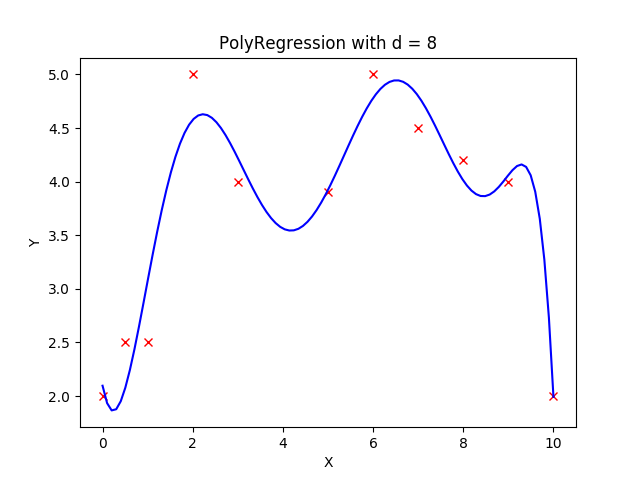
\includegraphics[width=150mm]{../hw1-code/results/a4.png}
\end{figure}

\begin{figure}[!ht]
  \centering
  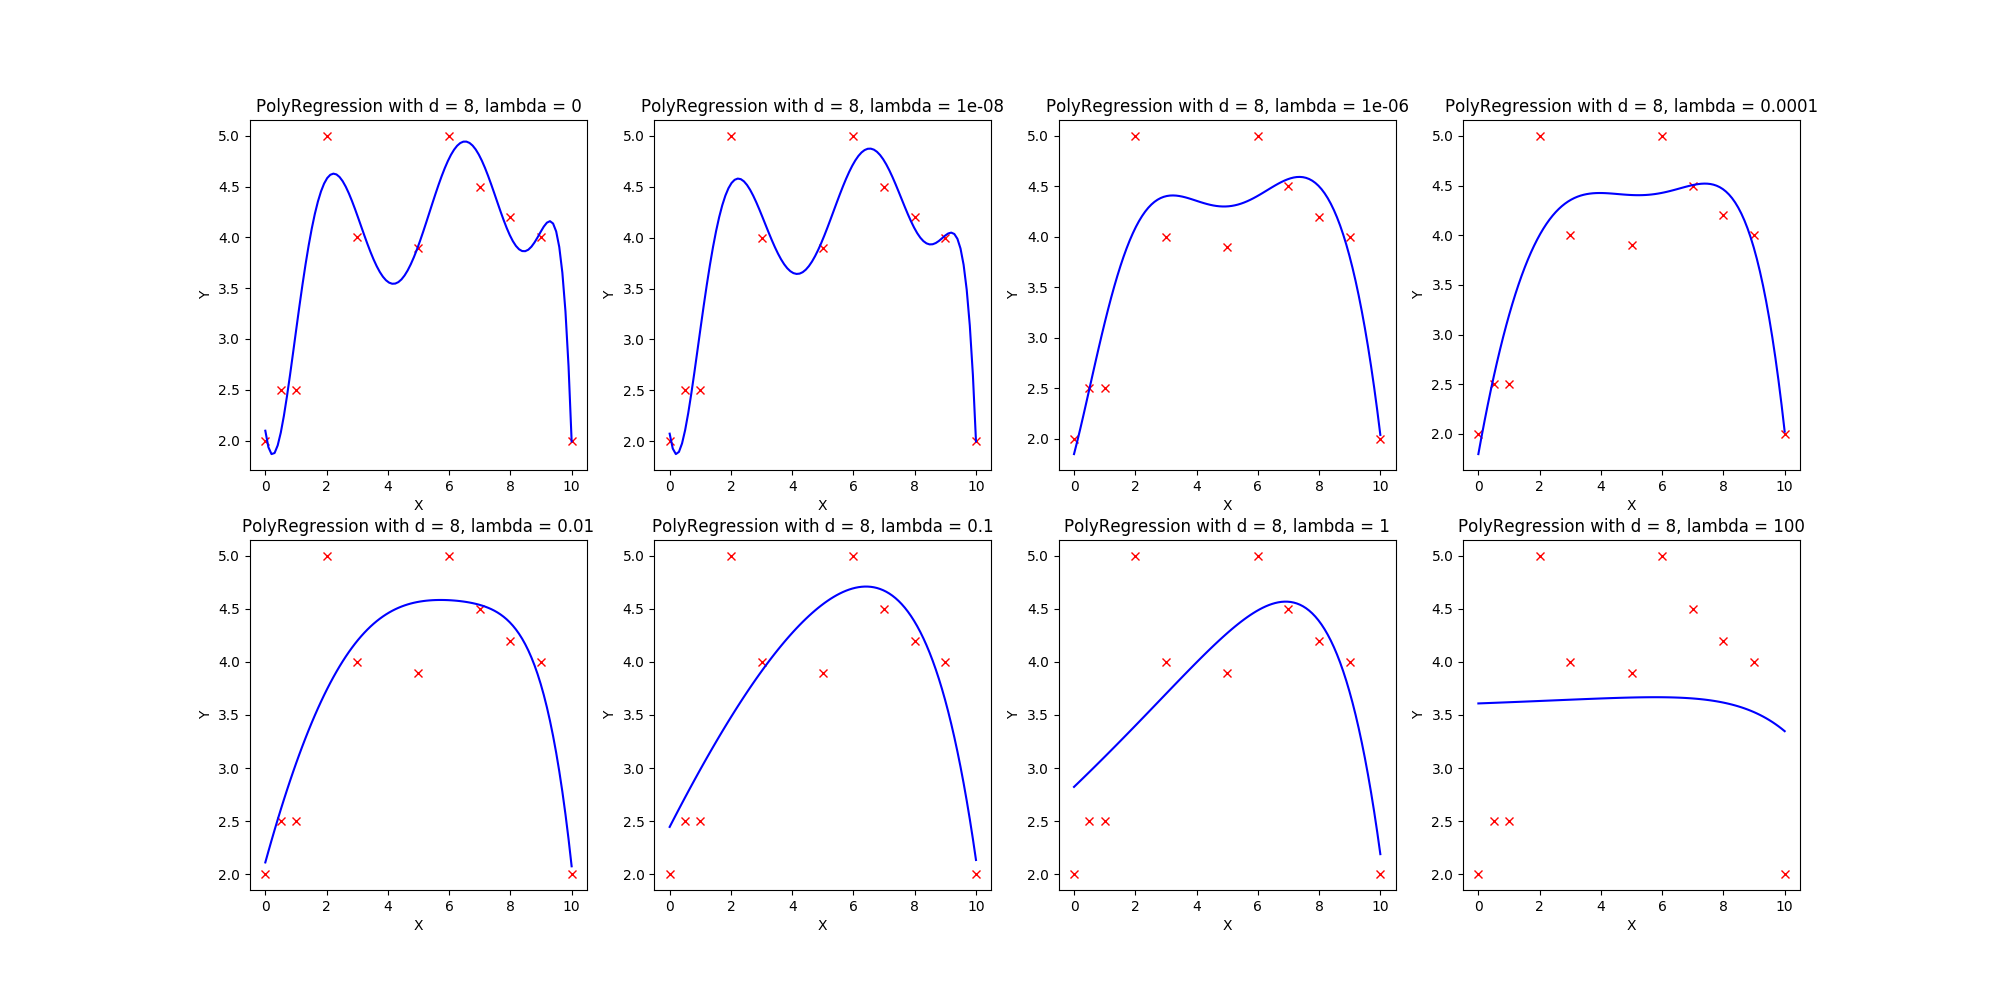
\includegraphics[width=218mm]{../hw1-code/results/a4_compilation.png}
\end{figure}

\newpage

}

\section*{A.5}
{\Large 

\begin{verbatim}
def calculate_error(n, calculated_values, actual_values):
  result = 0

  for i in range(n):
      result += np.square(calculated_values[i] - actual_values[i])

  return result / n

def learningCurve(Xtrain, Ytrain, Xtest, Ytest, reg_lambda, degree):
  """
  Compute learning curve

  Arguments:
      Xtrain -- Training X, n-by-1 matrix
      Ytrain -- Training y, n-by-1 matrix
      Xtest -- Testing X, m-by-1 matrix
      Ytest -- Testing Y, m-by-1 matrix
      reg_lambda -- regularization factor
      degree -- polynomial degree

  Returns:
      errorTrain -- errorTrain[i] is the training accuracy using
      model trained by Xtrain[0:(i+1)]
      errorTest -- errorTrain[i] is the testing accuracy using
      model trained by Xtrain[0:(i+1)]

  Note:
      errorTrain[0:1] and errorTest[0:1] won't actually matter, since we start displaying the learning curve at n = 2 (or higher)
  """

  n = len(Xtrain)
  m = len(Xtest)

  errorTrain = np.zeros(n)
  errorTest = np.zeros(n)

  #TODO -- complete rest of method; errorTrain and errorTest are already the correct shape

  model = PolynomialRegression(degree, reg_lambda)

  # Xtrain[0 : (i+1)]
  # Ytrain[0: (i+1)]

  for i in range(1, n):
      model.fit(Xtrain[0: (i+1)], Ytrain[0: (i+1)])

      errorTrain[i] = calculate_error(i + 1, model.predict(Xtrain[0: (i+1)]), Ytrain[0: (i+1)])
      errorTest[i] = calculate_error(m, model.predict(Xtest), Ytest)

  return errorTrain, errorTest
\end{verbatim}

\begin{figure}[ht!]
  \centering
  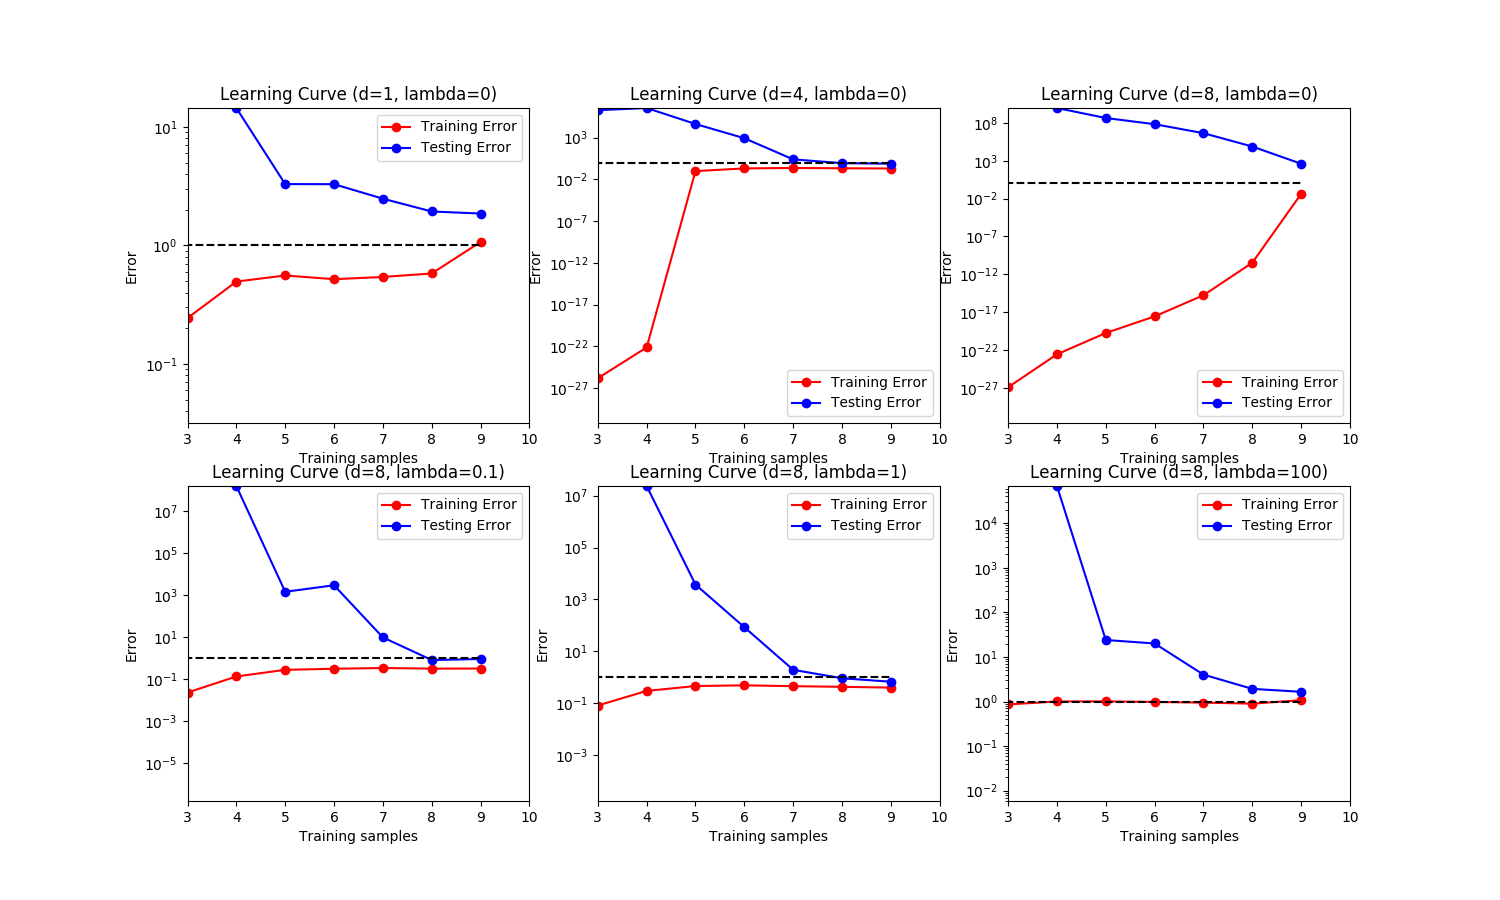
\includegraphics[width=215mm]{../hw1-code/results/a5.png}
\end{figure}

\newpage

}

\section*{A.6}
{\Large 

\subsection*{a.}

Show that $\widehat{W} = (X^TX + \lambda I)^{-1}X^TY$

\subsection*{b.}

I divided up , and got errors of . The code is as follows

\begin{verbatim}
\end{verbatim}

}

\end{document}